\chapter{Analysis}
\label{analysis}

\lettrine[lraise=0.1, nindent=0em, slope=-.5em]{\color{Violet}T}{his} chapter contains analytical part of the thesis, beginning with requirements analysis of the current situation, followed with analysis of the problems. Thereafter a requirement list for new e-course being established, followed by decision for methodology chosen for development of the e-course. 

\section{Problem Analysis}
\label{Problem Analysis}


Deficit of skilled \gls{ICT} specialist is known problem in Estonia \citep{website:ict_puudu} \citep{website:ict_needs}. However, several higher education institutes increased a number of spots in \gls{ICT} in theirs curricula, the number of graduated students is still insufficient for the field requirements\citep{website:TU_ict}, \citep{website:itc_facts}. Moreover, a continuous changing and of the field demands continually changes to curricula. Also a continuous learning are common in \gls{ICT} field because its changing. Therefore, a modernisation of the  \gls{ICT} curriculum and offering a continuous education courses are priority for \gls{EITC} to maintain professionalism as a graduated specialist.

To facilitate a curriculum development process the \gls{EISA} contacted with \gls{EITC} describing a problem: The deficiency of the skilled and security aware system administrators. Thereafter, provide initial proposal for solution to deal with the problem as seen in Appendix~\ref{Letter from CERT.EE to the Rector of Estonian IT College} on page ~\pageref{Letter from CERT.EE to the Rector of Estonian IT College}. However, instead of accepting the solution without questioning the curriculum heads of \gls{EITC} arranged several workshops for initial investigation of the problem and divided it to separate sub-problems and areas. For ensuring wider view of the problem several experts where involved from private companies, telecoms, banks, small business and start-ups. Author of this thesis characterize the proposal and establishes and negotiated the requirements for changes and composed an action plan.

Turing curricula development workshops author described the main reasons of the problem as following:

First, many system administrators acquired their knowledge through self-study. However, a continuous study is common in \gls{ICT} field the level of the specialist are unsteady and they do not have sufficient knowledge to build secure infrastructure.

Second, the applied education field do not provide qualification needed for managing secure infrastructure services. Therefore changes to curriculum are needed to fill the cap.

Third, in continuous education field is usual that private companies offer several courses for configuring and securing infrastructure, networks and services. However, those trainings are usually vendor based and focused heavily for promoting proprietary technologies without focusing broader knowledge in security field. 

Fourth, the system administrators in local government or municipal field have heterogeneous level of skills and knowledge. Therefore complication maintaining and helping them too difficult for \gls{CERT.EE}.

Fifth, all courses (needed to be developed) should be associated with the practical applicability of the theoretical knowledge and contain largely practical hands-on classes. Moreover, all materials should be based on not proprietary technology, like \gls{OpenBSD} or \gls{GNU/Linux}.

Sixth, the study program should focuses on practical learning by doing approach to \gls{ICT} subjects.
 Moreover, using virtual and game-like environments is a contemporary approach for teaching IT System administration and programming focusing to the cyber security requirements increases a motivation of students. Today the studies are too focused to the lecture form and practical classes are too simple and do not reflect the real situation.
 
For conclusion the security field in \gls{EITC} should be implemented by modifying existing courses and developing new subjects. Therefore, the author redesigns the IT system administration curricula in \gls{EITC} to mitigate the problems.



\section{Related Work}
\label{Related Work}
Designing an e-course is a challenge that has been solved by many lecturers and instructional developers. Moreover, the popularity of the cyber security related subjects in information and communications technology ICT curricula is growing and become a "student’s magnet" for higher educational institutes \citep{CyberIsHot}. Thereafter is possible to gain additional information by analysing related curricula and cyber security exercisers  in several higher educational institutes and analysing instructional design methodologies to achieve goals of this thesis. Moreover, to design practical course is also important to investigate courses given in region and in the world. However, is not possible to investigate a large amount of the courses and resources, the authors opinion is that by over-viewing several well known courses, trainings and challenges and articles the amount of gathered information is sufficient in minimal level for developing e-learning course.

\subsection{Cyber defence courses in Universities and Cyber exercisers}
Cyber defence exercisers can be categorized as practical exams and from suggested skill lists from those events can provide valuable information for curricula/course development process.

One comprehensive paper "Collective Views of the NSA/CSS Cyber Defense Exercise
on Curricula and Learning Objectives" about National Security describes how the National Security
Agency/Central Security Service (NSA/CSS) annual Cyber Defense Exercise (\gls{CDX}) influences curricula and studies at eight US federal service academies \citep{adams_CDX_curricula}. For example the Association for Computing Machinery (ACM) student can participate in \gls{CTF} exercisers and  visits to several security conferences \citep{adams_CDX_curricula}.

In University of Tartu several courses are related to topic as: Computer Security course  contains also 14 practical classes \footnote{Computer Security course   \url{https://courses.cs.ut.ee/2012/turve/fall/Main/HomePage} (2013-05-21)}, System Administration course gives good starting point with GNU/Linux and basic system administration \footnote{ System Administration course  \url{https://courses.cs.ut.ee/2013/syshald/spring/Main/Loengud} (2013-05-21)}
In University of Tartu have more security related courses but for this particular thesis those two are most important because they are practical and related to system administrators field.

In Tallinn University of Technology (\gls{TUT}) several courses are held as: Information Systems Hacking Attacks and Defence, Simulation of Attacks and Defense, Log Mining and Disk Forensics \footnote{wiki - lambda.ee \url{http://lambda.ee/wiki/Cyber_security_2012_second_year} (2013-05-21)}

Those courses are designed to give good hands-on experience on field for author opinion best courses in region. However, in \gls{EITC} all this material can not covered due curricula limitations but knowledge gathered on those courses will help to develop this particular e-learning course.

\subsection{Course in private companies and other organizations}

Two days course "Hands-on Hacking Essentials" given by Clarified Security OÜ contains Reconnaissance and information gathering, Privilege escalation, Jumping the (fire)wall, BackTrack 5, Remote exploitation, Attack Tool-sets \citep{website:clarifiedsecurity_hohe}. Therefore the given introduction should be a standard part of applied \gls{ICT} curricula. However, the course is too expensive to integrate it into \gls{EITC} curricula the lecturers are demonstrated the basics in several public and sometimes semi-private events organized by \gls{EISA}. Second course given by Clarified Security OÜ are the "Web Application security essentials" with duration of four days are focused to client side attacks and server side attacks giving systematic and well covered overview of the field \citep{website:clarifiedsecurity_hohe}.

However the both courses are designed keeping offensive in mind the basics should be covered also in \gls{EITC} curricula because to defend system also basic offensive knowledge and skills are required.

The SANS Institute organizes extensive security trainings also in online form \citep{website:SANS}. Moreover the institute shares free online resources for security topics \footnote{SANS - Reading Room \url{https://www.sans.org/reading_room/} (2013-05-21)} When developing a curriculum the topics and best practices from SANS Institute should be work through for clarifying learning outcomes and tools what can be used.

Last but not least the \gls{OWASP} project gives good and reusable study materials for theoretical and as well a practical guides as \gls{OWASP} Application Security Verification Standard (\gls{ASVS}) Project \footnote{\gls{OWASP}  (\gls{ASVS}) Project \url{https://www.owasp.org/index.php/Category:OWASP_Application_Security_Verification_Standard_Project} (2013-05-21)} 

\subsection{Large scale cyber security exercisers}
Several Cyber Defense Exercises (\gls{CDX}) are focused to train defence teams called Blue Team's \citep{website:NATO_CCD_COE,schepens_CDX}. And sometimes argued that \gls{CDX} is should be as a part of the any computer security curricula as addition to the classroom learning \citep{adams_CDX_curricula}. International Cyber Defence Exercise Locked Shields Locked Shields is defence exercise organised by NATO Cooperative Cyber Defence Centre of Excellence (\gls{NATO CCD COE}) and partners  \citep{website:NATO_CCD_COE}. 

The Blue Teams were the main training audience.
Expected Skillset blue team technicians from International Cyber Defence Exercise Locked Shields 2012 after action report \citep{website:NATO_CCD_COE}:
\begin{itemize}
\item Administration of Windows domain, Active Directory, Windows workstation
\item Administration of Linux servers like GNU/Debian and Ubuntu distributions
\item Firewalling (Netfilter based)
\item Knowledge about common network protocols/services and technologies as \gls{DNS}, \gls{NTP}, \gls{DHCP}, \gls{HTTP}, \gls{HTTPS}, \gls{SMTP}, \gls{POP3}, \gls{IMAP}, \gls{SSH}, \gls{FTP}, \gls{RADIUS}
\item \gls{KVM} virtualization platform
\item Web application technologies (\gls{HTML}, client-side and server-side scripting
such as JavaScript and \gls{PHP}, \gls{SQL} databases such as \gls{MySQL})
\item Administering of network devices (CISCO IOS, routing protocols)
\item Scripting skills in Perl
\end{itemize}

For large scale \gls{CDX} events the stability of the environment is always an issue \citep{website:NATO_CCD_COE,schepens_CDX}. Therefore, monitoring and IT service help are also fields that need investigation for environments where all students can start theirs virtual labs.

\section{Choosing Methodology for Developing an e-course}

Developing an e-course can be done without using design methodology but systematic approach should give more effective results. In principle the common systematic methods to develop an (e-learning) course are applying a Instructional System Design \gls{ISD} (sometimes cited as  Instructional Design \gls{ID}) model \citep{website:id_models}. However, several \gls{ISD} modes exists and can divided into three classes: behaviorism, cognitivist and prescriptive design \citep{website:id_models}, this thesis uses Prescriptive Design Model and specifically the \gls{ADDIE} process because method is used in Estonia and recommended for designing e-learning course \citep[p.~5]{OppeArenduskeskus2010}. Moreover, the \gls{ADDIE} model is not only good model that can be customized to meet specific needs, but ADDIE is a commonly used effective model for instructional  design \citep{ieee_addie_1607206}.

The methodology used to develop this e-course should encourage student activity in learning process. Moreover student should have possibility to choice learning speed, -place and -time. Today's students have different learning style and background and methodology should reckon with individual differences.

Developed e-course should support people with disabilities. In \gls{EITC} several people have hearing disabilities and all important material should presented also without audio. For example in screen casts videos all important information should be written also in screen or added as transcript.

Today’s learning environment should support student communities where students can act as mentors and also feel part on the study program. Course integration with student driven initiative like forums, blogs, wiki pages and other collaboration learning methods should be possible and not restricted.

 However, the \gls{ADDIE} model has several weaknesses as being too waterfall type model because it is not iterative \citep{website:weakesses_of_ADDIE_model}. Alternatively The Dick and Carey Model are used to design instructions \citep{dick2005systematic}. However, the Estonian guide to for design a quality-grade e-learning course based on \gls{ADDIE} model \citep{OppeArenduskeskus2010}. Although the ADDIE model is not modelling anything and technically should it called a \gls{ISD} framework \citep{bichelmeyer2004addie}, in this thesis term ADDIE model is used because this name is commonly known and used for designing e-learning courses \citep{bichelmeyer2004addie, OppeArenduskeskus2010}.
For conclusion the \gls{ADDIE} model was chosen to develop particular cyber security e-learning course and model itself is described in the next section.

\subsection{The ADDIE Model}

The \gls{ADDIE} model is used for creating different types of instructions as courses, trainings \citep{website:addie, lohr1998using}. Moreover, the ADDIE method is  used to provide a systematic, iterative course development process with feedback-based approach to improve quality of study \citep{website:using_addie}.

The ADDIE model contain five stages: Analysis, Desing, Development, Implementation and Evaluation as seen in illustration~\ref{figure:the addie model} \citep{website:addie}



\begin{figure}[H]
 \centering 
 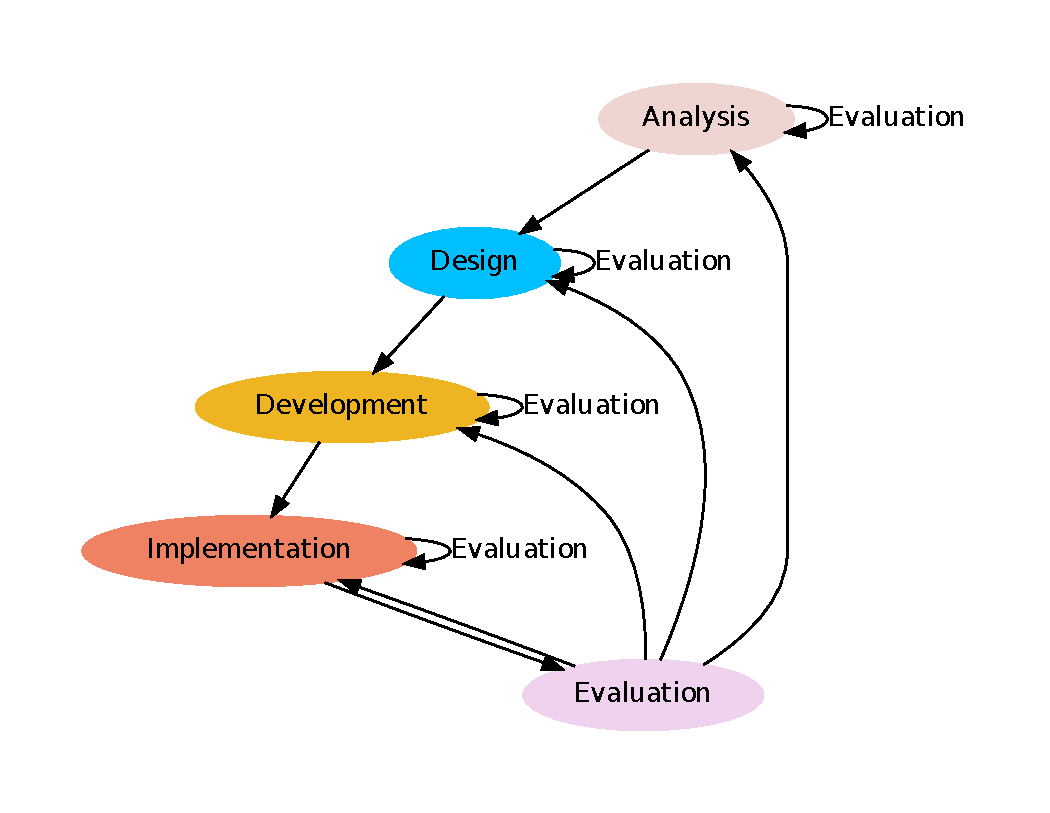
\includegraphics[width=0.6\textwidth]{addie_model.pdf}
 \rule{35em}{0.5pt} 
 \caption{The ADDIE model} 
 \label{figure:the addie model} 
\end{figure}

Firstly, the goal of the analysis phase is for investigation of the gap between goal and
existing situation. Therefore, this phase investigates instructional goals, current situation, learner, objectives \citep{chen2007learning, website:addie}.

Secondly, the design phase focuses following areas; assessments design, learning content, learning strategies and course format \citep{chen2007learning, website:addie}.


Thirdly, the work of development includes creating of course materials, choosing methodology and technologies, testing of material using run-through with small group. \citep{OppeArenduskeskus2010, website:addie, chen2007learning}.


Fourthly, the implementation stage is describes implementing the above work of three previous steps and gives possibility to evaluate full course in evaluation phase \citep{chen2007learning, website:addie}.


Finally, the evaluation phase is for assessing of the learning effect through evaluation. However the evaluation process takes place in every stage as seen in illustration~\ref{figure:the addie model} the final evaluation focuses whole course and focuses to the feedback from students and lecturers and output of this phase is valuable for next courses \citep{OppeArenduskeskus2010, website:addie}.

\section{Analysis of the e-learning course}
According to \gls{ADDIE} model the analysis stage establishes goals for the course and evaluation of the current situation and strategy for implementing goals followed by analysis of the learners and the content of the course \citep{website:addie}

The analysis phase of the \gls{ADDIE} model contains four sub-phases \citep{website:addie}.
\begin{enumerate}
\item Instructional Goals -- main objective plan for new course
\item Instructional Analysis -- analysis of the current situation
\item Learner Analysis -- target group properties like previous knowledge about the field
\item Learning Outcomes -- list of knowledges and skills to achieve instructional goals
\end{enumerate}


\subsection{Instructional Goals}
The Instructional Goals and learning objectives should established before designing new course and they give answer to the student questions: Why should I study this topic and what I learn during this and how I will evaluated? \citep{website:addie}


The instructional goals for new course were established using interviews with \gls{EISA} and several companies. Therefore where listed technologies needed to know by system administrators. Moreover, the additional input fore establishing goals come form analysis of the current curriculum.

The list of discussed topics is too big to give full list even in appendices. After listing all possible topic all items got priorities. However, the list of topics was still too long to cover it in three year college. Although first prioritizing working group divided topics to smaller groups and divided it into three areas. First, topics what should cover private companies providing product based training. Second, topics what are not suitable for three year education and cant be efficiently integrated into study program like subjects already given in \gls{TUT} or in \gls{UT}. Third, the topics what are suitable for \gls{EITC}

The instructional goals for the e-learning course: firstly, give an introduction of IT infrastructure services, secondly, give skills and knowledge for installing and configuring of IT infrastructure services, thirdly give knowledge and skills for protecting IT infrastructure services. Moreover, give knowledge and skills for documenting IT infrastructure services.

\subsection{Instructional Analysis}
The Instructional Analysis should answer the question: What steps are necessary to achieve  established instructional goals and what tools are needed? \citep{website:addie}.

To achieve this goal the study focuses on hands-on practical classes combined with lecturers and seminars. Moreover,to achieve maximum impact of the course, all content and methodology are designed to be suitable in classroom learning and using e-learning or blended learning which is combination of e-learning and classroom activities. Moreover, materials are designed to support self-study in e-learning form.

The name of the new course: Securing IT Infrastructure Services. However the course is not yet included into curricula the subject program will be discussed on board in June 2013 and in case positive feedback the new course will be held on Spring 2014.

New e-learning course should be given on second course at spring semester preluded with course I233 - Operating System Administration\footnote{Curriculum subject I233 \url{https://itcollege.ois.ee/en/curriculum-subject/view?curriculum_id=2&subject_id=130&year=2012}}. However, the continuous education students should pass pre-sessional entry course which covers basics of GNU/Linux course as seen in Appendix~\ref{Preliminary course - dpkg based GNU/Linux} or pass the entry theory test with questions on Table~\ref{tab:preliminary_test} on page \pageref{tab:preliminary_test} and a practical test listed in Table~\ref{tab:preliminary_practical_test} on page~\pageref{tab:preliminary_practical_test}.

\subsubsection{Analysing of the requirements, scope and restrictions for e-course}
During several curricula development seminars author establishes requirements for this particular e-course according to input from partners like \gls{EISA}, students feedback, graduate students feedback and curricula analysis from other higher educational institutes and private training companies. 

Because of main target groups are \gls{EITC} students and IT system administrators who need knowledge and skills for defending their system the course must developed according to their needs and reckon with theirs previous background and knowledge. However, for students it means pre-requirement course list but for system administrators it means preliminary course if they need it. Therefore, the preliminary tests for entering the course are needed to gain required skills with GNU/Linux and if possible also include BSD family in basic level because OpenBSD is used in \gls{EISA} project S4A.
The curricula development and authoring a learning materials are funded by EU therefore they  published using licensing terms allows to use materials for teaching the subject and also derive new work if license stays the same.
Today EITC hands-on labs on GNU/Linux are done using one or two virtual machines but to simulate more realistic situations in laboratory scenarios the number of supportive virtual machines should be more. For example to perform lab “configuring e-mail service” a student needs fours virtual machines. One client, MTA - configured by student, DNS -  configured by student, Other preconfigured MTA and pre configured DNS. For conclusion to provide more realistic lab scenario some pre-configured virtual machines are needed for each lab type or even for each student and this is hard setup for student itself.

Final main requirements are following:
\begin{enumerate}[label=Requirement \arabic*.,leftmargin=*]
  \item Developed e-course must be usable for \gls{EITC} students and also in continuous education field for system administrators
  \item Course must contain pre-sessional entry course to GNU/Linux and should cover basics  of the OpenBSD/FreeBSD systems
  \item Course should contains main aspects of system administration and focus to the defence of the systems
  \item Developed course materials should released using Creative Commons \gls{CC-BY-SA} license
  \item Laboratory work should be as realistic as possible including needed infrastructure to run complex infrastructure services. Therefore required solution for set-up hands-on environment in class or home.
\end{enumerate}

Choosing technical tools, establishing learning outcomes and authoring learning materials will follow those requirements and instructional goals.

\subsection{Learner analysis}


The analysis of the target group provided valuable input to the course development because starting point of the course and difficulty level of the hands-on labs depends on the target group level and course content should fill the cap between knowledge/skills of the target group and instructional goals. Therefore, analysis of the target group is needed to design efficient e-learning course.

 According to problem analysis the target group can divided to two separate groups, the students who do not have long working experience and system administrators who have working experience in particular field but often do not have degree or diploma in \gls{ICT} field or they are graduated several years ago.

The first target group are second and third years students who already mastered basics of operating systems, GNU/Linux administration and Windows administration. The second target group are system administrators with different background because of deep specializing in enterprises. Common relevant (on course development point of view)  properties are described in Table~\ref{tab:targetgroup}. However, the ethnic, gender and age is out of investigation because irrelevance for designing this course.

\begin{table}[h]
\centering
\caption{The target group properties}

\begin{tabular}{|p{4cm}|p{5cm}|p{5cm}|}
\hline 
\color{blue}
Property & \color{blue} Students & \color{blue} System Administrators \\ 
\hline 
Background & No or few work experience in field & Experience on one or more specialized field \\ 
\hline 
Motivation & To get diploma and valuable work also knowledge/skills needed to protect \gls{ICT} systems & To get knowledge and skills to protect \gls{ICT} systems \\ 
\hline 
Time and possibilities & possible to do home work/reading & in practice can not do homework/readings efficiently  \\ 
\hline 
Previous knowledge & From \gls{EITC} (GNU/Linux, Windows)  &  heterogeneous, some people are very skilled and some are very weak on field. Most of people do not have proper GNU/Linux experience.  \\ 
\hline 
Previous study experience & Good & Lesser \\ 
\hline 
Study Stile & Student's style (everything done little before deadlines) & All study should take place during contact hours  \\ 
\hline 
How homogeneous the group are (knowledge and skills) & More flat & heterogeneous \\ 
\hline 
Previous experience in GNU/Linux & Enough to start the course & Poor (only 10\%) passed the theory test~\ref{Preliminary Tests}  \\ 
\hline 
\end{tabular} 

\label{tab:targetgroup}
\end{table}
 
Is possible that studying cyber security affects student behaviour for example using learned methodologies to attack live systems. Therefore, special disclaimer need to be added to labs that have also offensive aspects.
 
For conclusion to the analysis of target group's can stated that course material should be suitable for both groups. First group, the students have advantage because having sufficient time for home readings. However the second group has advantage from previous work experience. Second group's problem is insufficient knowledge about GNU/Linux system and separate short auxiliary course about basic command line is needed before entering to the main course. However some system administrators do not need those course and need for additional course will decided using entry test developed during this thesis.


\subsection{Learning Outcomes}

By establishing learning outcomes the goals of the course should elaborate on and get more specific form. Therefore, they should give impression what to expect from course to the student and composed  \citep[p.~7]{OppeArenduskeskus2010}.

The learning outcomes with threshold criteria described in Table~\ref{tab:learning_outcomes}.

% Students are able to demonstrate common attacks against web applications and explain attacks against \gls{DNS} (or using it for attack) as well able to explain terms \gls{VPN}, \gls{SAN}, \gls{NAS}, \gls{IDS}, \gls{IPS}. Moreover the students able to document installed services.

\begin{table}[h]
\centering
\caption{Learning Outcomes}
{ \small
\begin{tabular}{|p{7cm}|p{7cm}|}

\hline 
\color{blue} Learning Outcome &\color{blue}  Threshold criteria -- minimal level required to pass \\ 
\hline 

\hline 
After completing the e-learning course all students will be able to install, configure and secure  IT infrastructure services as \gls{NTP}, \gls{DNS}, \gls{DHCP}, web servers, firewalls, file servers and authentication services. & Participant installs and configures services and explain configuration choices done during the practical task according to lab scenario.\\ 
\hline 
Student is able to explain basic terms of \gls{NTP}, \gls{DNS}, \gls{DHCP}, web servers, firewalls, file servers and authentication services. 
& 

Student is able to explain basic concept of \gls{NTP}, \gls{DNS}, \gls{DHCP}, web servers and  basic terminology of IT infrastructure services.
\\ 
\hline 
Student are able to secure web and file services and \gls{NTP}, \gls{DNS}, \gls{DHCP} servers.

& 
Student installs, configures and secures services according lab guide.
\\ 
\hline 
Student are able to test simpler attacks against web services and measure the successiveness of the attack.

& Student demonstrates attacks against web services and explains the result and impact of each attack \\ 
\hline 
Student are able to install central authentication services using prepared guide.
& 
Student configures central authentication system (LDAP, Kerberos, SAMBA4) and client machine to authenticate using central system
\\
\hline 
Student are able to explain following IT infrastructure subjects as: VPN, virtualization, SQL, SAN/NAS/CAS, monitoring, logging, IDS and IPS
& 
Student are able to define and explain IT infrastructure terminology.
\\ 

\hline 
Student are able to document IT infrastructure service according to documentation instruction guide

& 

Student are able do compose documentation of one service according to documentation guidelines. 
\\ 
\hline 

\end{tabular} 
}
\label{tab:learning_outcomes}
\end{table}

Designed learning outcomes do not describe every lab and theirs objectives. However, the good learning material needs learning objectives that support the achieve the established learning outcomes. However, sometimes learning outcomes and learning objects defined as the same, but in this thesis the objectives are more detailed then learning outcomes \citep{website:objective_vs_outcome}.

\section{Evaluation of Analysis stage}

Accordingly to the \gls{ADDIE} model the evaluation for each stage should performed according to following aspectsseen in Table~\ref{tab:evoluation_analysis} \citep[p.~11]{OppeArenduskeskus2010}. Therefore the evaluation of analysis phase done by self-assessment and peer-assessment methodology according to Estonian e-learning course quality guide assessment matrix \citep{website:quality_mx}.

Evaluation of the analysis phase given in Table~\ref{tab:evoluation_analysis} and it is in questionnaire format with grade scale: One, the quality requirement is not met. Two, the quality requirement is partly met. Three, the quality requirement is mostly met. Four, the quality requirement is fully met.

\begin{table}[h]
\centering
\caption{The evaluation of the analysis stage }
{ \small 
\begin{tabular}{|p{6cm}|p{2cm}|p{5cm}|}
\hline 
\color{blue} Evoluation question & \color{blue} Result [1..4] & \color{blue} Comments and references \\ 
\hline
E-learning course corresponds to needs and capabilities of the target group? 
& 4  &  preliminary course fills the cap (Self-assessment)\\ 
\hline 
Does course have institutional goal and learning outcomes established a point of student view?
& 4 & Self-assessment  \\ 
\hline 
Does e-learning suits the course and are properly explained?
& 2 & Suits but not specially explained Self-assessment \\ 
\hline
Does a course content bind to learning outcomes and reckon with context of e-learning?
& 3 & Course content is releated with learning outcomes but not specially for e-learning Self-assessment \\ 
\hline 
\end{tabular} 
}
\label{tab:evoluation_analysis}
\end{table}

Although, the this was self-assessment and peer-assessment the Steering Committee of Curricula will assess the Subject Program seen in Appendix~\ref{appendix:SubjecProgram} on summer 2013.

%{\color{red} 
%Kas kursus vastab sihtrühma vajadustele ja võimalustele?
%
%Kas kursusel on eesmärk ja õppijakeskselt sõnastatud õpiväljundid?
%
%Kas e-õppe vormi kasutamine kursusel on põhjendatud?
%
%Kas kursuse sisu vastab õpiväljunditega ja arvestab e-õppe kontekstiga?
%}\citep[p.~11]{OppeArenduskeskus2010}

